\documentclass[addpoints, answers, 11pt, a4paper]{exam}

% Packages
\usepackage{color}
\usepackage[colorlinks]{hyperref}
\usepackage{graphicx}
\usepackage{amssymb}
\usepackage{amsmath}


% Styling of worksheet
\renewcommand{\familydefault}{\sfdefault}
\pointsinrightmargin
\marginpointname{~\points}
\pointpoints{pt}{pts}

\pagestyle{headandfoot}
\firstpageheader{
	Assignment 6: Bayesian Networks \\ Deadline: December 3, 2023 (\numpoints~points)
}
{}
{%
	Name:~\fillin[\myname][5cm] \\Student number:~\fillin[\mystudentnumber][5cm]%
}

\runningheader{Page \thepage\ of \numpages}{}{Student number:~\fillin[\mystudentnumber][4cm]}
\runningheadrule

\firstpagefooter{}{}{}
\runningfooter{}{}{}

\SolutionEmphasis{\itshape\color{blue}}
\CorrectChoiceEmphasis{\itshape\color{blue}}

\renewenvironment{TheSolution}
{\par}
{}

\newcommand*{\multiplevalid}{\checkboxchar{$\square$}}
\newcommand*{\onevalid}{\checkboxchar{$\bigcirc$}}
\newcommand*{\checkbox}[1][]{\ifx&#1&\choice\else\CorrectChoice\fi}

% Useful formatting commands 
\newcommand*{\prob}[1]{\ensuremath{\mathsf{P}(#1)}}
\newcommand*{\indep}{\ensuremath{\perp \!\!\! \perp}}


% Student information
\newcommand*{\myname}{Jason Liu}
\newcommand*{\mystudentnumber}{s0213082}

\begin{document}	
	\begin{questions}
		
		\fullwidth{\section*{Probability (\pointsinrange{probability} points)}}
		\begingradingrange{probability}
		
		\fullwidth{
			\raisebox{-0.5\height}{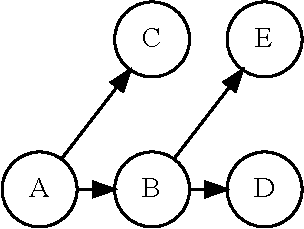
\includegraphics[width=.3\linewidth]{res/probabilities_net}}
			\hspace{1em}
			\raisebox{-0.4\height}{\vbox{
				\begin{tabular}{|c|c|}
					\hline
					& \prob{A} \\
					\hline
					$+a$ & 0.25 \\
					$-a$ & 0.75 \\
					\hline
				\end{tabular}		
				\begin{tabular}{|c|c|c|}
					\hline
					\prob{B \mid A} & $+b$ & $-b$ \\
					\hline
					$+a$ & 0.5 & 0.5 \\
					$-a$ & 0.25 & 0.75 \\
					\hline
				\end{tabular}
				\begin{tabular}{|c|c|c|}
					\hline
					\prob{C \mid A} & $+c$ & $-c$ \\
					\hline
					$+a$ & 0.2 & 0.8 \\
					$-a$ & 0.6 & 0.4 \\
					\hline
				\end{tabular}
				\\[1em]
				\begin{tabular}{|c|c|c|}
					\hline
					\prob{D \mid B} & $+d$ & $-d$ \\
					\hline
					$+b$ & 0.6 & 0.4 \\
					$-b$ & 0.8 & 0.2 \\
					\hline
				\end{tabular}
				\begin{tabular}{|c|c|c|}
					\hline
					\prob{E \mid B} & $+e$ & $-e$ \\
					\hline
					$+b$ & 0.25 & 0.75 \\
					$-b$ & 0.1 & 0.9 \\
					\hline
				\end{tabular}
			}}
		}
		\vspace{1em}

		\question[2] Using the Bayes net and conditional probability tables above, calculate the following quantities:
		
		% TODO: Fill in
		\begin{parts}
			\part \prob{+b \mid +a}			= \fillin[0.5]
			\part \prob{+a, +b}				= \fillin[\prob{+a}\prob{+b \mid +a}$=\dfrac{1}{8}$]
			\part \prob{+a \mid +b}			= \fillin[$\prob{+a \mid +b} = \dfrac{\prob{+b \mid +a} \prob{+a}}{\prob{+b \mid +a}\prob{+a} + \prob{+b \mid -a}\prob{-a}} = \dfrac{0.5 * 0.25}{0.5 * 0.25 + 0.25 * 0.75} = \dfrac{2}{5}$]
			\part \prob{-e, +a}				= \fillin[$0.25*(0.5 * 0.75 + 0.5 * 0.9) = 0.20625$]
			\part \prob{D \mid A} =
				\begin{solution}
					\begin{tabular}{|c|c|c|}
						\hline
						\prob{D \mid A} & $+d$ & $-d$ \\
						\hline
						$+a$ & $\dfrac{7}{40}$ & $\dfrac{3}{40}$ \\
						$-a$ &  $\dfrac{36}{160}$ & $\dfrac{15}{80}$  \\
						\hline
					\end{tabular}
				\end{solution}
		\end{parts}
		\endgradingrange{probability}
		
		
		\fullwidth{\section*{Independence (\pointsinrange{independence} points)}}
		\begingradingrange{independence}
		
		\multiplevalid
		\question[4] For each of the following equations, select the minimal set of conditional independence assumptions necessary for the equation to be true.
		
		\begin{parts}
			\part $\prob{A, C} = \prob{A \mid B} \prob{C}$ \vspace{.5em}
			
			\begin{oneparcheckboxes}		% TODO: Fill in (\checkbox[1] for true)
				\checkbox[x] $A \indep B$
				\checkbox[] $A \indep B \mid C$
				\checkbox[x] $A \indep C$
				\checkbox[] $A \indep C \mid B$ \\
				\checkbox[] $B \indep C$
				\checkbox[] $B \indep C \mid A$
				\checkbox[] No independence assumptions needed
			\end{oneparcheckboxes} \\
			
			\part $\prob{A \mid B, C} =\frac{\prob{A}\prob{B \mid A}\prob{C \mid A}}{\prob{B \mid C}\prob{C}} $ \vspace{.5em}
			
			\begin{oneparcheckboxes}
				\checkbox[] $A \indep B$
				\checkbox[] $A \indep B \mid C$
				\checkbox[] $A \indep C$
				\checkbox[] $A \indep C \mid B$ \\
				\checkbox[] $B \indep C$
				\checkbox[x] $B \indep C \mid A$
				\checkbox[] No independence assumptions needed
			\end{oneparcheckboxes} \\
			
			\part $\prob{A, B} = \sum_{c}\prob{A \mid B, c}\prob{B | c}\prob{c} $ \vspace{.5em}
			
			\begin{oneparcheckboxes}
				\checkbox[] $A \indep B$
				\checkbox[] $A \indep B \mid C$
				\checkbox[] $A \indep C$
				\checkbox[] $A \indep C \mid B$ \\
				\checkbox[] $B \indep C$
				\checkbox[] $B \indep C \mid A$
				\checkbox[x] No independence assumptions needed
			\end{oneparcheckboxes} \\
			
			\part $\prob{A, B \mid C, D} = \prob{A \mid C, D}\prob{B \mid A, C, D}$ \vspace{.5em}
			
			\begin{oneparcheckboxes}
				\checkbox[] $A \indep B$
				\checkbox[] $A \indep B \mid C$
				\checkbox[] $A \indep C$
				\checkbox[] $A \indep C \mid B$ \\
				\checkbox[] $B \indep C$
				\checkbox[] $B \indep C \mid A$
				\checkbox[x] No independence assumptions needed
			\end{oneparcheckboxes}
		\end{parts}
		
		
		\newpage
		\onevalid
		\question[4] Indicate whether each of the following conditional independence relationships is guaranteed to be true in the Bayes Net below. If the independence relationship does not hold, identify all active (d-connected) paths in the graph.
		\label{q:dseparation}
		
		{\centering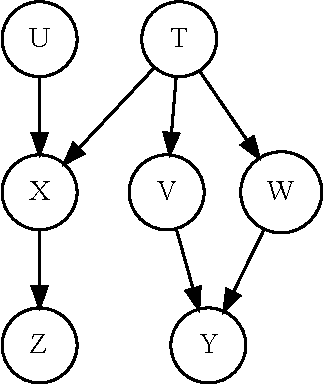
\includegraphics[width=.3\linewidth]{res/separation} \\}
		
		\begin{parts}
			\part $T \indep Y$ \\
			Independence is
			\begin{oneparcheckboxes}		% TODO: Fill in (\checkbox[1] for true)
				\checkbox[] Guaranteed \checkbox[x] Not Guaranteed
			\end{oneparcheckboxes}
			\begin{solution}
				% If not guaranteed, enter active paths:
				$T \rightarrow V \rightarrow Y$\\
				$T \rightarrow W \rightarrow Y$
				
			\end{solution} \vspace{1em}
			
			\part $T \indep Y \mid W$ \\
			Independence is
			\begin{oneparcheckboxes}
				\checkbox[] Guaranteed \checkbox[x] Not Guaranteed
			\end{oneparcheckboxes}
			\begin{solution}
				% If not guaranteed, enter active paths:
				$T \rightarrow V \rightarrow Y$
				
			\end{solution} \vspace{1em}
			
			\part $U \indep T$ \\
			Independence is
			\begin{oneparcheckboxes}
				\checkbox[x] Guaranteed \checkbox[] Not Guaranteed
			\end{oneparcheckboxes}
			\begin{solution}
				% If not guaranteed, enter active paths:
				
			\end{solution} \vspace{1em}
			
			\part $U \indep T \mid Z$ \\
			Independence is
			\begin{oneparcheckboxes}
				\checkbox[] Guaranteed \checkbox[x] Not Guaranteed
			\end{oneparcheckboxes}
			\begin{solution}
				% If not guaranteed, enter active paths:
				$((U \rightarrow X)$ and $(T \rightarrow X)) \rightarrow Z$ because $Z$ is a decendant of $X$ and $X$ forms a v-structure.
				While $Z$ is observed, the v-structure is active.
			\end{solution} \vspace{1em}
			
			\part $Z \indep U$ \\
			Independence is
			\begin{oneparcheckboxes}
				\checkbox[] Guaranteed \checkbox[x] Not Guaranteed
			\end{oneparcheckboxes}
			\begin{solution}
				% If not guaranteed, enter active paths:
				$U \rightarrow X$
			\end{solution} \vspace{1em}
			
			\part $Z \indep Y \mid V$ \\
			Independence is
			\begin{oneparcheckboxes}
				\checkbox[] Guaranteed \checkbox[x] Not Guaranteed
			\end{oneparcheckboxes}
			\begin{solution}
				% If not guaranteed, enter active paths:
				$T \rightarrow X \rightarrow Z$\\
				$T \rightarrow W \rightarrow Y$\\
				$X \leftarrow T \rightarrow W$
				
			\end{solution} \vspace{1em}
			
			\part $Z \indep Y \mid T, W$ \\
			Independence is
			\begin{oneparcheckboxes}
				\checkbox[x] Guaranteed \checkbox[] Not Guaranteed
			\end{oneparcheckboxes}
			\begin{solution}
				% If not guaranteed, enter active paths:
				
			\end{solution} \vspace{1em}
			
			\part $Z \indep W$ \\
			Independence is
			\begin{oneparcheckboxes}
				\checkbox[] Guaranteed \checkbox[x] Not Guaranteed
			\end{oneparcheckboxes}
			\begin{solution}
				% If not guaranteed, enter active paths:
				$T \rightarrow X \rightarrow Z$\\
				$X \leftarrow T \rightarrow W$
				
			\end{solution} \vspace{1em}
		\end{parts}
		\endgradingrange{independence}
		
		
		\newpage
		\fullwidth{\section*{Representation (\pointsinrange{representation} points)}}
		\begingradingrange{representation}
		
			\multiplevalid
			\question[4] We are given the following ten Bayes nets, labeled $\mathbf G_1$ to $\mathbf G_{10}$:

			{\centering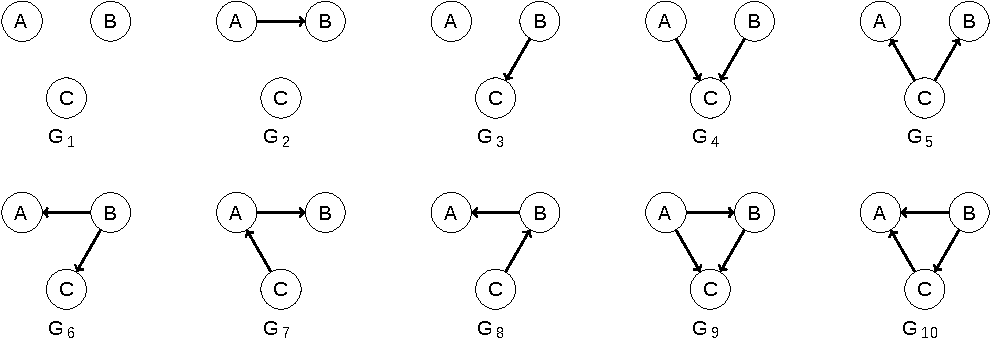
\includegraphics[width=.9\linewidth]{res/nodes1} \\}

			and the following three Bayes nets, labeled $\mathbf B_1$ to $\mathbf B_3$:
			
			{\centering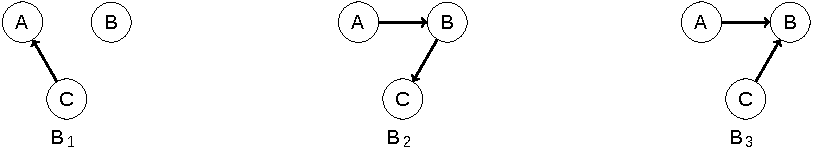
\includegraphics[width=0.7\linewidth]{res/nodes2} \\}
			
			\vfill
			
			\begin{parts}
				\part Assume we know that a joint distribution $d_1$ (over $A$, $B$, $C$) can be represented by Bayes net $\mathbf B_1$. Mark all of the following Bayes nets that are guaranteed to be able to represent $d_1$.
				
				\begin{oneparcheckboxes}		% TODO: Fill in (\checkbox[1] for true)
					\checkbox[] $G_1$
					\checkbox[] $G_2$
					\checkbox[] $G_3$
					\checkbox[x] $G_4$
					\checkbox[x] $G_5$
					\\
					\checkbox[] $G_6$
					\checkbox[x] $G_7$
					\checkbox[] $G_8$
					\checkbox[x] $G_9$
					\checkbox[x] $G_{10}$
					\\
					\checkbox[] None of the above
				\end{oneparcheckboxes} \\
				
				\part Assume we know that a joint distribution $d_2$ (over $A$, $B$, $C$) can be represented by Bayes net $\mathbf B_2$. Mark all of the following Bayes nets that are guaranteed to be able to represent $d_2$.
				
				\begin{oneparcheckboxes}
					\checkbox[] $G_1$
					\checkbox[] $G_2$
					\checkbox[] $G_3$
					\checkbox[] $G_4$
					\checkbox[] $G_5$
					\\
					\checkbox[x] $G_6$
					\checkbox[] $G_7$
					\checkbox[x] $G_8$
					\checkbox[x] $G_9$
					\checkbox[x] $G_{10}$
					\\
					\checkbox[] None of the above
				\end{oneparcheckboxes} \\
			
				\part Assume we know that a joint distribution $d_3$ (over $A$, $B$, $C$) \textbf{cannot} be represented by Bayes net $\mathbf B_3$. Mark all of the following Bayes nets that are guaranteed to be able to represent $d_3$.
				
				\begin{oneparcheckboxes}
					\checkbox[] $G_1$
					\checkbox[] $G_2$
					\checkbox[] $G_3$
					\checkbox[] $G_4$
					\checkbox[] $G_5$
					\\
					\checkbox[] $G_6$
					\checkbox[] $G_7$
					\checkbox[] $G_8$
					\checkbox[x] $G_9$
					\checkbox[x] $G_{10}$
					\\
					\checkbox[] None of the above
				\end{oneparcheckboxes} \\
			
				\part Assume we know that a joint distribution $d_4$ (over $A$, $B$, $C$) can be represented by Bayes nets $\mathbf B_1$, $\mathbf B_2$ and $\mathbf B_3$. Mark all of the following Bayes nets that are guaranteed to be able to represent $d_4$.
				
				\begin{oneparcheckboxes}
					\checkbox[x] $G_1$
					\checkbox[x] $G_2$
					\checkbox[x] $G_3$
					\checkbox[x] $G_4$
					\checkbox[x] $G_5$
					\\
					\checkbox[x] $G_6$
					\checkbox[x] $G_7$
					\checkbox[x] $G_8$
					\checkbox[x] $G_9$
					\checkbox[x] $G_{10}$
					\\
					\checkbox[] None of the above
				\end{oneparcheckboxes}
			\end{parts}
		\endgradingrange{representation}
		
		
		\newpage
		\fullwidth{\section*{Inference (\pointsinrange{inference} points)}}
		\begingradingrange{inference}

			\question[4] Using the same Bayes Net from question~\ref{q:dseparation}, we want to compute $\prob{Y \mid +z}$. All variables have binary domains. Assume we run variable elimination to compute the answer to this query, with the following variable elimination ordering: $U, T, X, V, W$.
			
			Complete the following description of the factors generated in this process:
			
			\begin{parts}
				\part After inserting evidence, we have the following factors to start out with: \\
				$ \prob{U}, \prob{T}, \prob{X \mid U, T}, \prob{V \mid T}, \prob{W \mid T}, \prob{+z \mid X}, \prob{Y \mid V, W} $ \vspace{1em}
				
				\part When eliminating $U$ we generate a new factor $f_1$ as follows, which leaves us with the factors:
				$f_1(X, T) = \sum_{u} \prob{u}\prob{X \mid u, T}$ \\
				Factors: $\prob{T}, \prob{V \mid T}, \prob{W \mid T}, \prob{+z \mid X}, \prob{Y \mid V, W}, f_1(X, T)$ \vspace{1em}
				
				\part When eliminating $T$ we generate a new factor $f_2$ as follows, which leaves us with the factors:
				
				\begin{solution}		% TODO: Fill in
					$f_2(V, W, X) = \sum_{t} \prob{t}\prob{V \mid t}\prob{W \mid t} f_1(X, t)$ \\
					Factors: $\prob{+z \mid X}, \prob{Y \mid V, W}, f_2(V, W, X)$
				\end{solution} \vspace{1em}
			
				\part When eliminating $X$ we generate a new factor $f_3$ as follows, which leaves us with the factors:
				
				\begin{solution}
					$f_3(+z, V, W) = \sum_{x} \prob{+z \mid x} f_2(V, W, x) $ \\
					Factors: $\prob{Y \mid V, W}, f_3(+z, V, W)$
				\end{solution} \vspace{1em}
			
				\part When eliminating $V$ we generate a new factor $f_4$ as follows, which leaves us with the factors:
				
				\begin{solution}
					$f_4(+z, W, Y) = \sum_{v} \prob{Y \mid v, W} f_3(+z, v ,W)$ \\
					Factors: $f_4(+z, W, Y)$
				\end{solution} \vspace{1em}
			
				\part When eliminating $W$ we generate a new factor $f_5$ as follows, which leaves us with the factors:
				
				\begin{solution}
					$f_5(+z, Y) = \sum_{w} f_4(+z, w, Y)$ \\
					Factors: $f_5(+z, Y)$
				\end{solution} \vspace{1em}
			
				\part How would you obtain $\prob{Y \mid +z}$ from the factors left above?

				\begin{solution}
					$\prob{Y \mid +z} = \dfrac{f_5(+z, Y)}{\sum_{y} f_5(+z, y)}$ \\
				\end{solution} \vspace{1em}
				
				\part What is the size of the largest factor that gets generated during the above process?
				
				\begin{solution}
					The largest factor will be $f_2(V, W, X)$, which has size $2^3 = 8$.
				\end{solution} \vspace{1em}
			
				\part Does there exist a better elimination ordering (one which generates smaller largest factors)? Argue why not or give an example.
				
				\begin{solution}
					Yes, there exists a better elimination ordering.
					For example, if we eliminate $X$ before $T$, then the largest factor will be $f_1(X, T)$, which has size $2^2 = 4$.
				\end{solution} \vspace{1em}
			\end{parts}
		\endgradingrange{inference}
	
	\end{questions}
\end{document}